% 05-nguon-luc.tex — Chương 5: Nguồn lực và tiến độ

\chapter{Nguồn lực và tiến độ}\label{ch:nguonluc}

\section{Nguồn lực con người}

Sáng kiến cần sự phối hợp của bốn nhóm; vai trò được phân định như sau:

{\tablefont
\begin{longtable}{@{}L{3.6cm}>{\raggedright\arraybackslash}p{8.81cm} L{2.8cm}@{}}
\caption{Vai trò các nhóm tham gia}\label{tab:vaitro}\\
\toprule
\hdrrow\hh{Nhóm} & \hh{Trách nhiệm chính} & \hh{Nhân sự}\\
\midrule
\endfirsthead
\toprule
\hdrrow\hh{Nhóm} & \hh{Trách nhiệm chính} & \hh{Nhân sự}\\
\midrule
\endhead
\bottomrule
\endfoot
Data Scientist & Thiết kế chỉ số, quy tắc nhãn, huấn luyện, đánh giá mô hình; theo dõi chất lượng kết quả; giải thích cho nghiệp vụ. & \phc{số người}\\
\rowa Data Enineer & Cung cấp dữ liệu nguồn và nhãn thực tế theo lịch; bảo đảm đúng cấu trúc, mã hóa định danh; báo trước khi thay đổi cột/định dạng. & \phc{số người}\\
Chăm sóc khách hàng & Sử dụng danh sách; liên hệ khách hàng; ghi nhận kết quả và nguyên nhân thực tế; xác nhận nhãn. & \phc{số người}\\
\rowa Vận hành hạ tầng & Quản lý máy chủ, cơ sở dữ liệu, container, sao lưu, phân quyền truy cập. & \phc{số người}\\
\end{longtable}}
\vspace{4pt}

\section{Nguồn lực công nghệ}

Sáng kiến tận dụng hạ tầng và công cụ đã có: cơ sở dữ liệu PostgreSQL, máy chủ chạy container, bộ điều phối Apache Airflow, kho đóng gói nội bộ.
Các thư viện phân tích dữ liệu sử dụng đều là phần mềm mã nguồn mở. Không có hạng mục mua sắm phần mềm bản quyền nào được nêu trong tài liệu dự án.

{\tablefont
\begin{longtable}{@{}L{4.2cm}>{\raggedright\arraybackslash}p{11.43cm}@{}}
\caption{Nguồn lực công nghệ sử dụng}\label{tab:congnghe}\\
\toprule
\hdrrow\hh{Hạng mục} & \hh{Mô tả}\\
\midrule
\endfirsthead
\toprule
\hdrrow\hh{Hạng mục} & \hh{Mô tả}\\
\midrule
\endhead
\bottomrule
\endfoot
Cơ sở dữ liệu & PostgreSQL nội bộ, tổ chức theo nhiều ngăn dữ liệu (xem Bảng~\ref{tab:schema}).\\
\rowa Điều phối công việc & Apache Airflow 3.1.7 chạy dưới dạng container.\\
Phân tích và mô hình & Bộ thư viện phân tích dữ liệu và học máy mã nguồn mở (xử lý dữ liệu, mô hình, tối ưu tham số, giải thích kết quả).\\
\rowa Thư mục dữ liệu trên máy chủ & Thư mục nhận tệp dữ liệu đầu vào, thư mục xử lý, thư mục nhật ký.\\
Kho đóng gói nội bộ & Lưu phiên bản đóng gói của hệ thống để triển khai và hoàn tác.\\
\end{longtable}}
\vspace{4pt}

\section{Tiến độ triển khai}

Tiến độ được trình bày theo giai đoạn. Các giai đoạn đã xây dựng căn cứ vào tài liệu bàn giao hệ thống; các giai đoạn tiếp theo là đề xuất.

\begin{figure}[!ht]
\centering
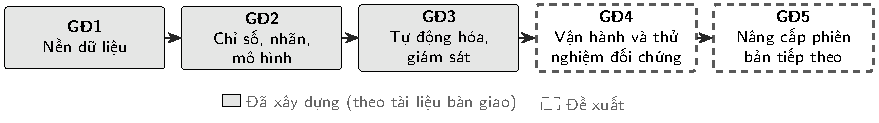
\includegraphics[width=421.7bp]{figures/fig08.pdf}
\caption{Các giai đoạn triển khai}\label{fig:giaidoan}
\end{figure}

{\tablefont
\begin{longtable}{@{}L{1.0cm}L{3.2cm}>{\raggedright\arraybackslash}p{5.56cm}L{2.4cm}L{2.2cm}@{}}
\caption{Nội dung, sản phẩm và trạng thái từng giai đoạn}\label{tab:tiendo}\\
\toprule
\hdrrow\hh{GĐ} & \hh{Tên} & \hh{Sản phẩm chính} & \hh{Trạng thái} & \hh{Thời gian}\\
\midrule
\endfirsthead
\toprule
\hdrrow\hh{GĐ} & \hh{Tên} & \hh{Sản phẩm chính} & \hh{Trạng thái} & \hh{Thời gian}\\
\midrule
\endhead
\bottomrule
\endfoot
1 & Nền dữ liệu & Quy trình nạp tệp đơn hàng, tổng hợp, hợp đồng, khiếu nại, nhãn thực tế; chuẩn hóa cấu trúc; kiểm tra độ mới và đầy đủ. & Đã xây dựng & \phc{~}\\
\rowa 2 & Chỉ số, nhãn, mô hình & Bảng nền dài hạn; bảng chỉ số cửa sổ; bộ nhãn thống nhất; lọc điều kiện; mô hình cơ sở và mô hình chính; tinh chỉnh; đánh giá theo thời gian. & Đã xây dựng & \phc{~}\\
3 & Tự động hóa và giám sát & Sáu luồng công việc Airflow; xét duyệt mô hình; chấm điểm và xuất danh sách; lý do rủi ro; giám sát độ lệch; dọn dẹp định kỳ. & Đã xây dựng & \phc{~}\\
\rowa 4 & Vận hành và thử nghiệm đối chứng & Đưa danh sách vào quy trình chăm sóc; đo mức nền; chạy thử nghiệm đối chứng; báo cáo hiệu quả. & Đề xuất & \phc{~}\\
5 & Nâng cấp phiên bản tiếp theo & Quản lý vòng đời mô hình; giám sát trực quan; kiểm tra lại trong quá khứ; các kỹ thuật bổ sung. & Đề xuất & \phc{~}\\
\end{longtable}}
\vspace{4pt}

\section{Mốc nghiệm thu đề xuất}

{\tablefont
\begin{longtable}{@{}L{3.6cm}>{\raggedright\arraybackslash}p{12.03cm}@{}}
\caption{Mốc nghiệm thu và tiêu chí}\label{tab:nghiemthu}\\
\toprule
\hdrrow\hh{Mốc} & \hh{Tiêu chí nghiệm thu}\\
\midrule
\endfirsthead
\toprule
\hdrrow\hh{Mốc} & \hh{Tiêu chí nghiệm thu}\\
\midrule
\endhead
\bottomrule
\endfoot
M1 -- Dữ liệu sẵn sàng & Dữ liệu các nguồn được nạp đúng lịch; kiểm tra độ mới và đầy đủ đạt.\\
\rowa M2 -- Mô hình đạt chuẩn & Mô hình qua rào chắn an toàn; có số liệu F1, độ chính xác cảnh báo, độ bao phủ trên bài thi cuối kỳ.\\
M3 -- Vận hành tự động & Chuỗi nạp $\rightarrow$ chỉ số $\rightarrow$ chấm điểm chạy liên tục nhiều chu kỳ không cần can thiệp tay.\\
\rowa M4 -- Giá trị kinh doanh & Thử nghiệm đối chứng cho thấy nhóm áp dụng giữ được nhiều đơn hàng/doanh thu hơn nhóm đối chứng.\\
\end{longtable}}
\vspace{4pt}
